% !Mode:: "TeX:UTF-8"
\chapter{正文编写}
\echapter{How to write}

本章节介绍了如何插入公式、图片、表格、引用等。

\section{插入图片}
\esection{How to Insert a Figure}

\begin{figure}[htbp]
\centering
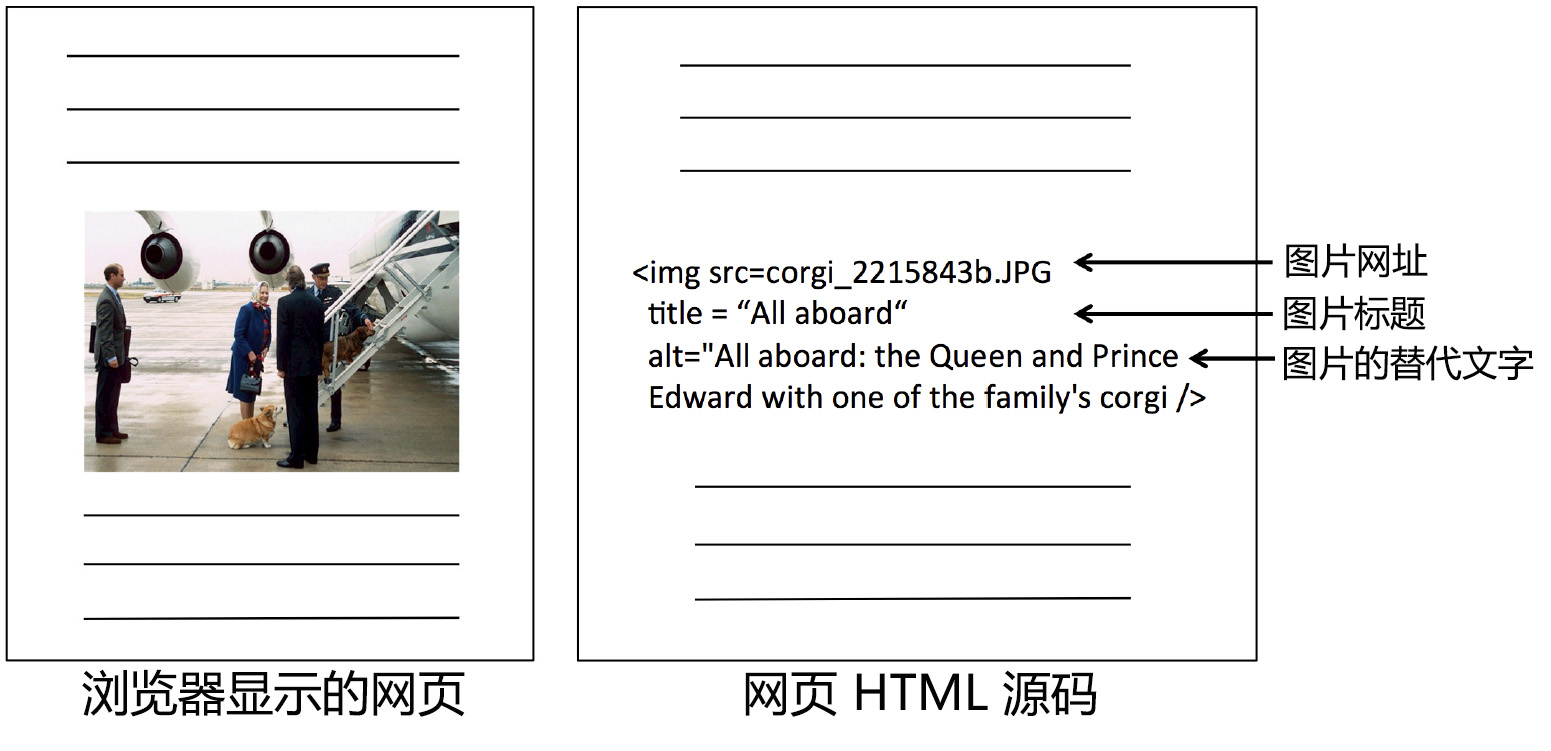
\includegraphics[width=0.8\textwidth]{htmltext.jpg}
\caption{图片在网页中的显示}
\label{FIGhtmltext}
\end{figure}

使用\verb|figure|标记,设置宽度、图片文件名、标题、标签。

插入子图片:

\begin{figure}[htbp]
\centering
\subfloat[GIST]{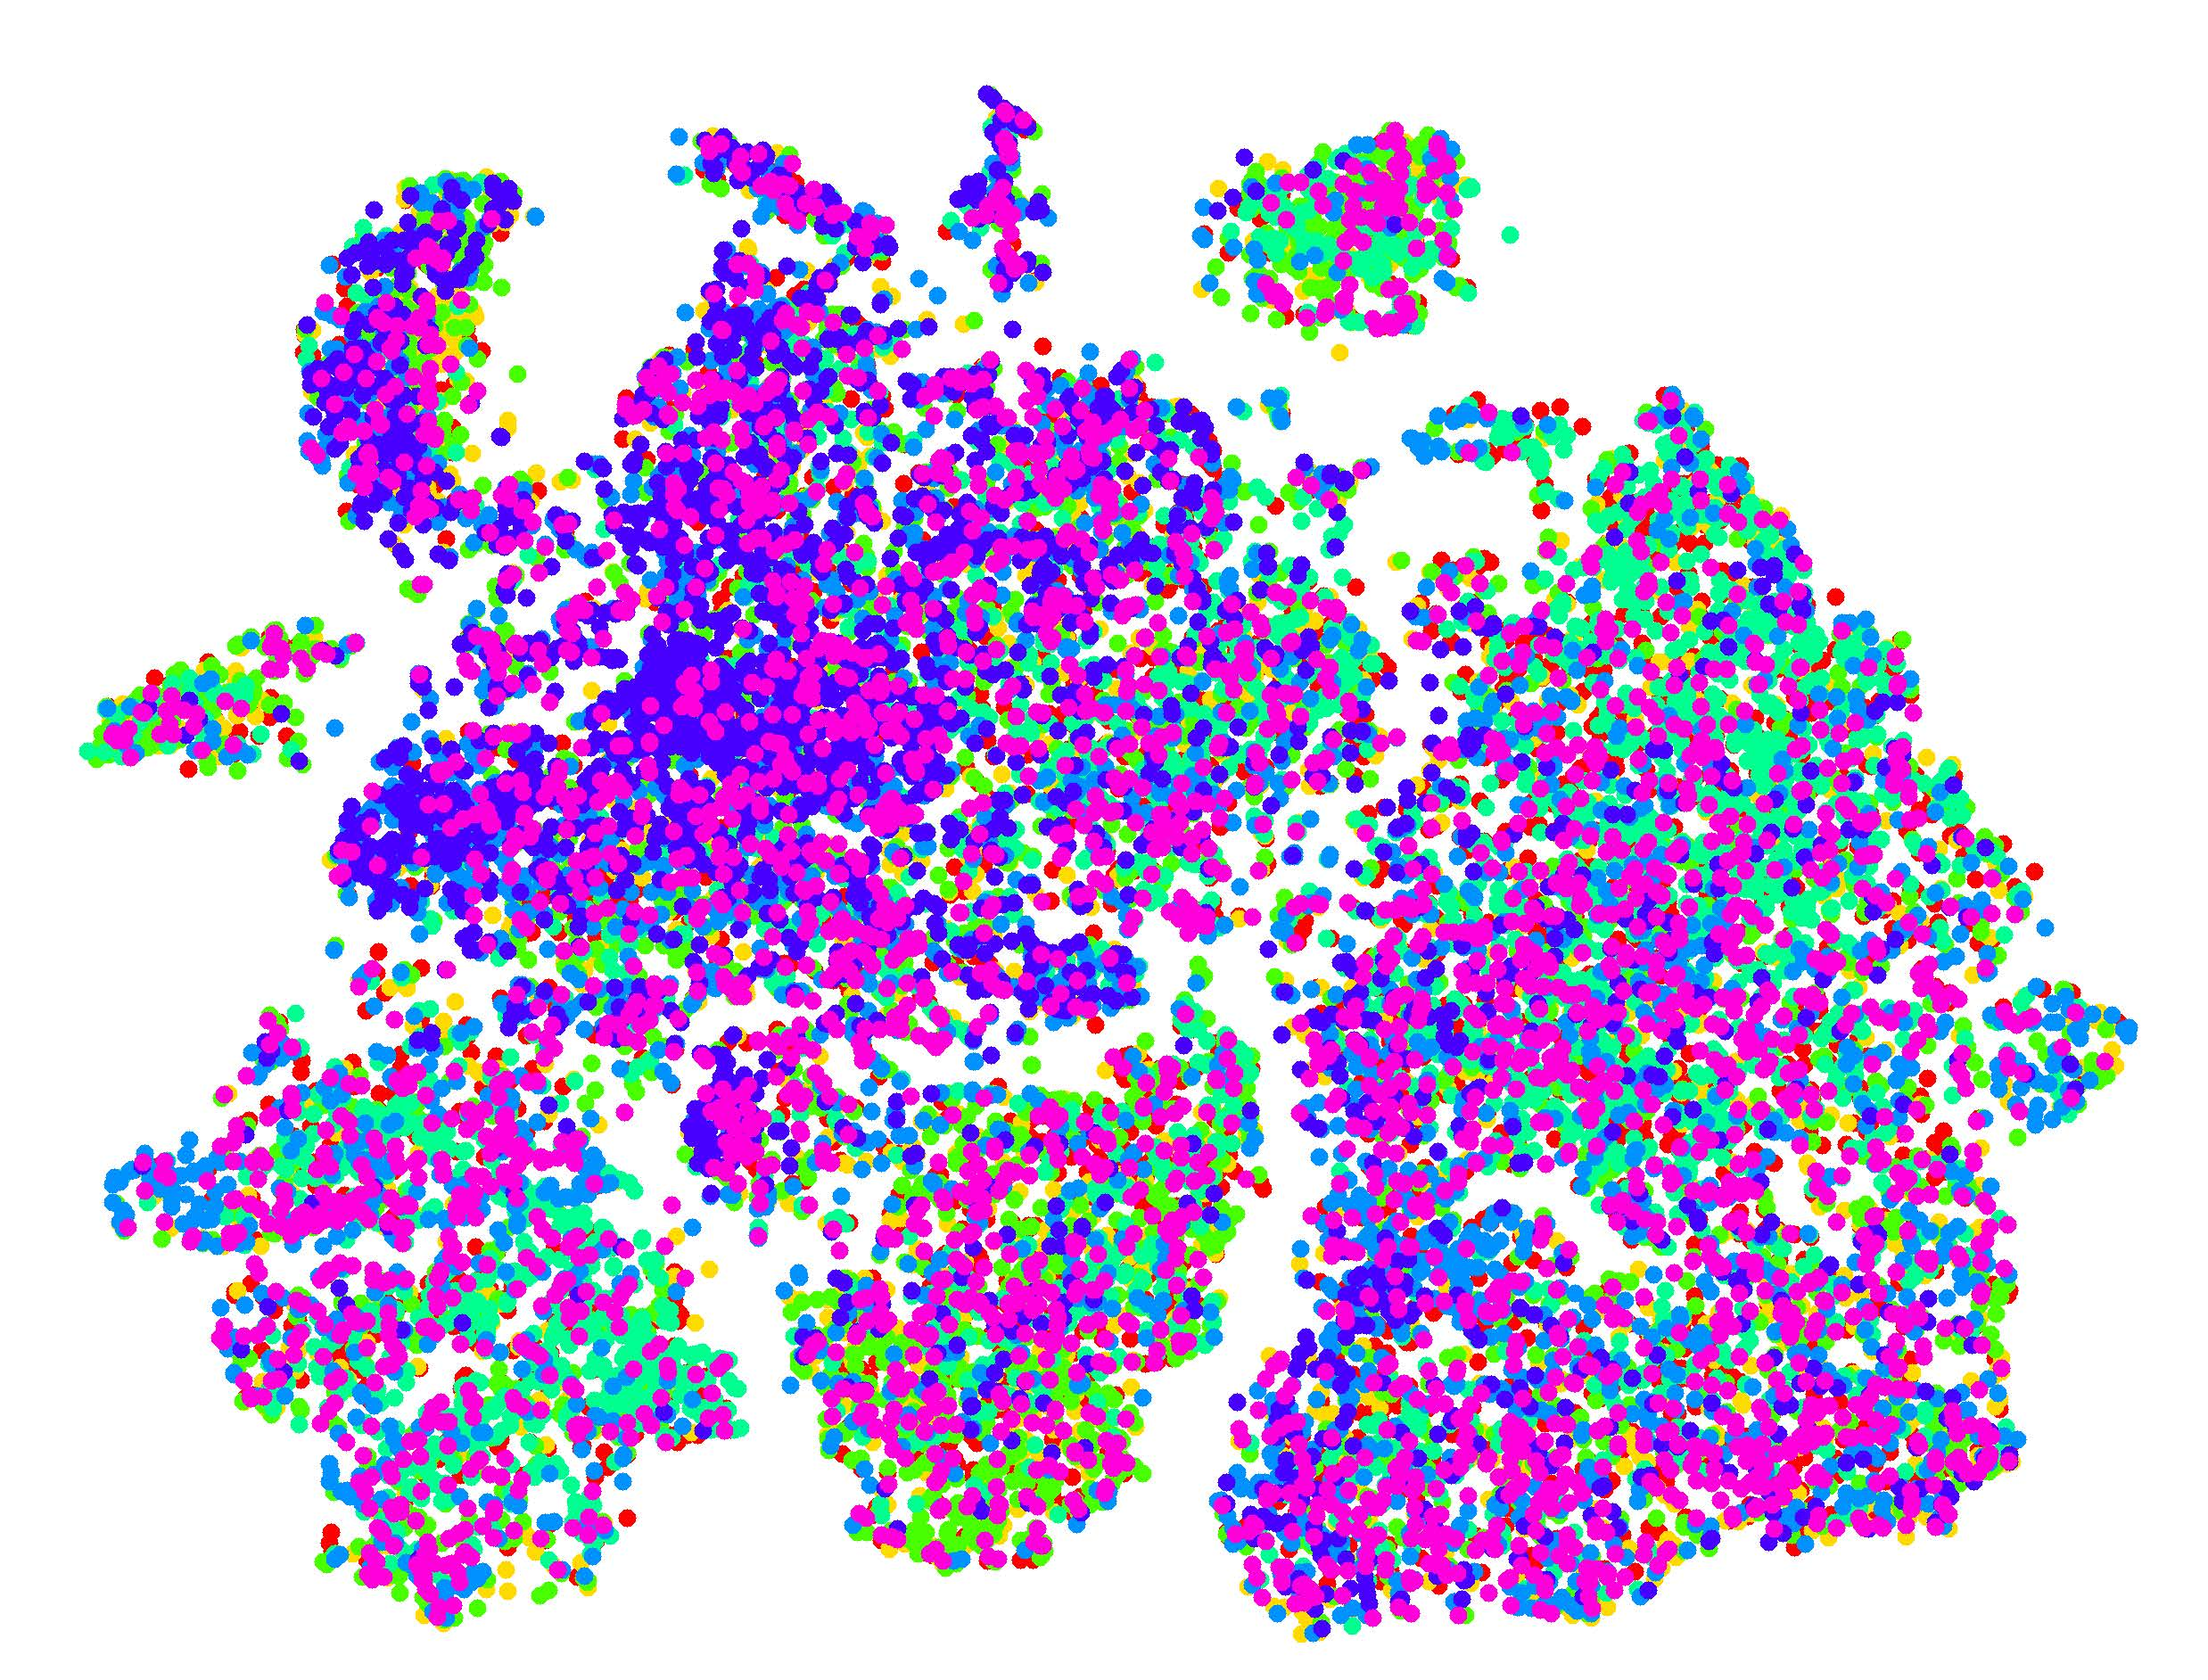
\includegraphics[width=0.3\textwidth]{GIST.jpg}}
~~
\subfloat[DeCAF$_1$]{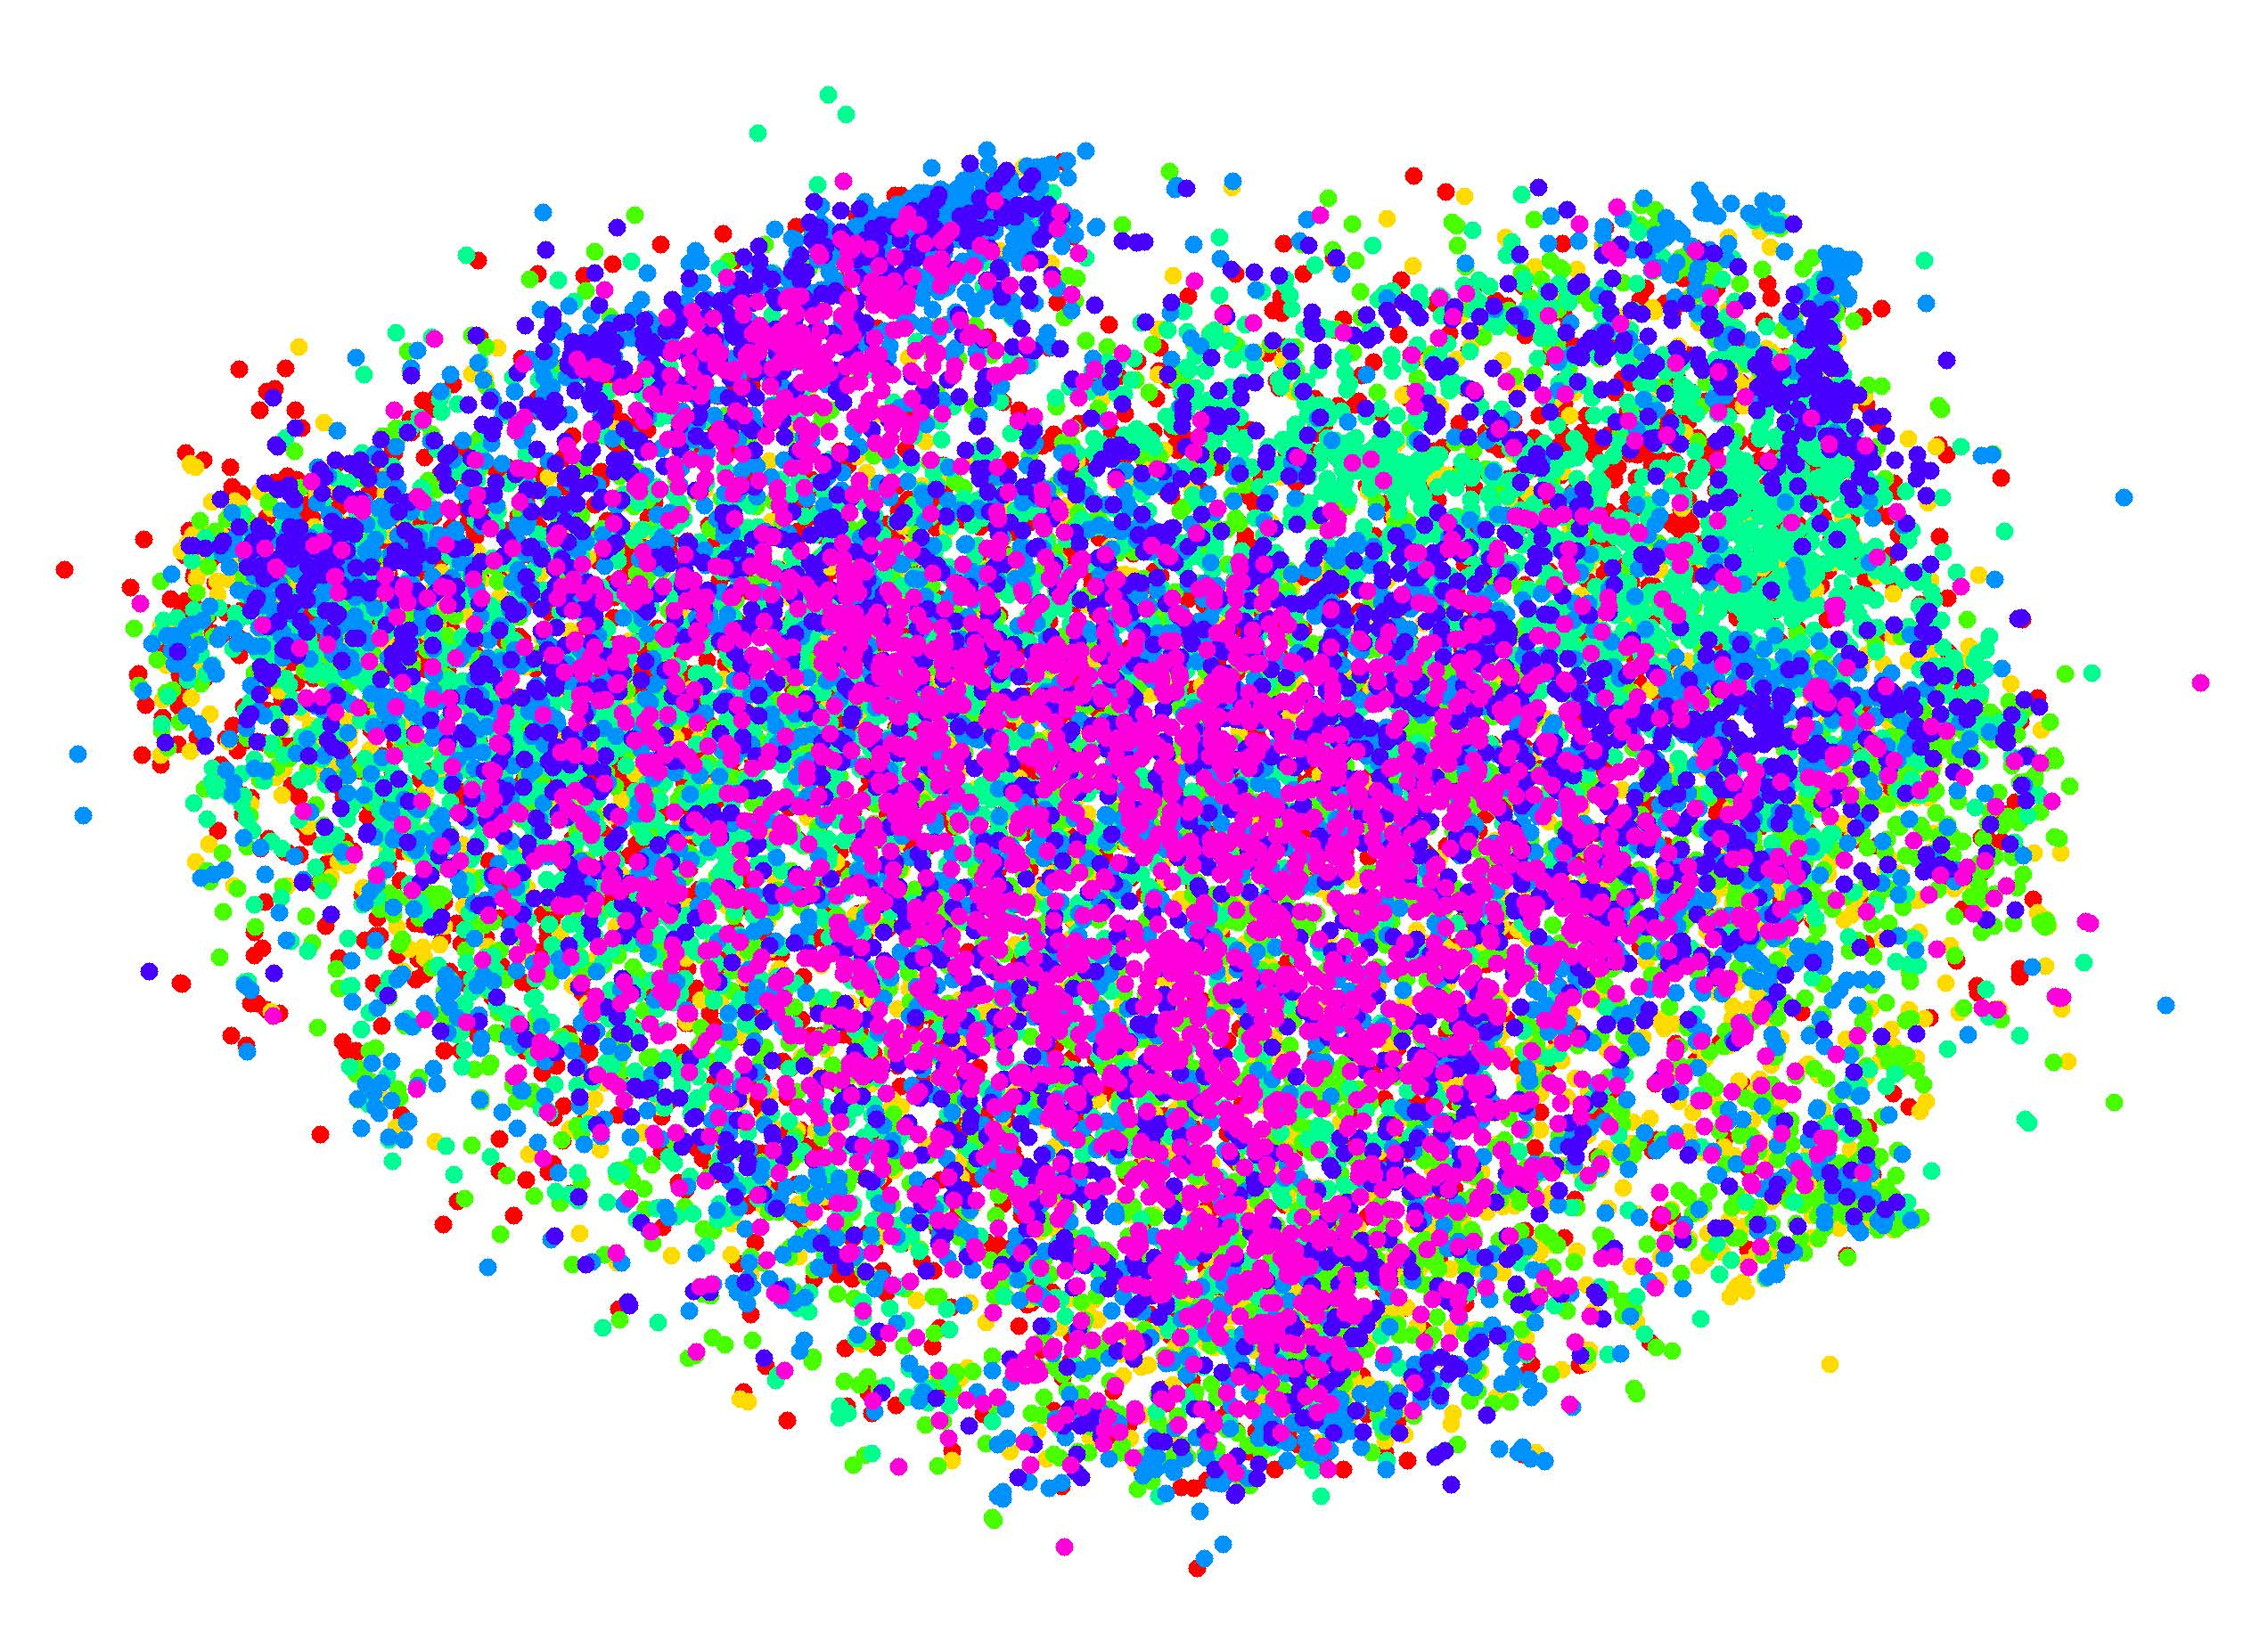
\includegraphics[width=0.3\textwidth]{DECAF1.jpg}}
~~
\subfloat[DeCAF$_6$]{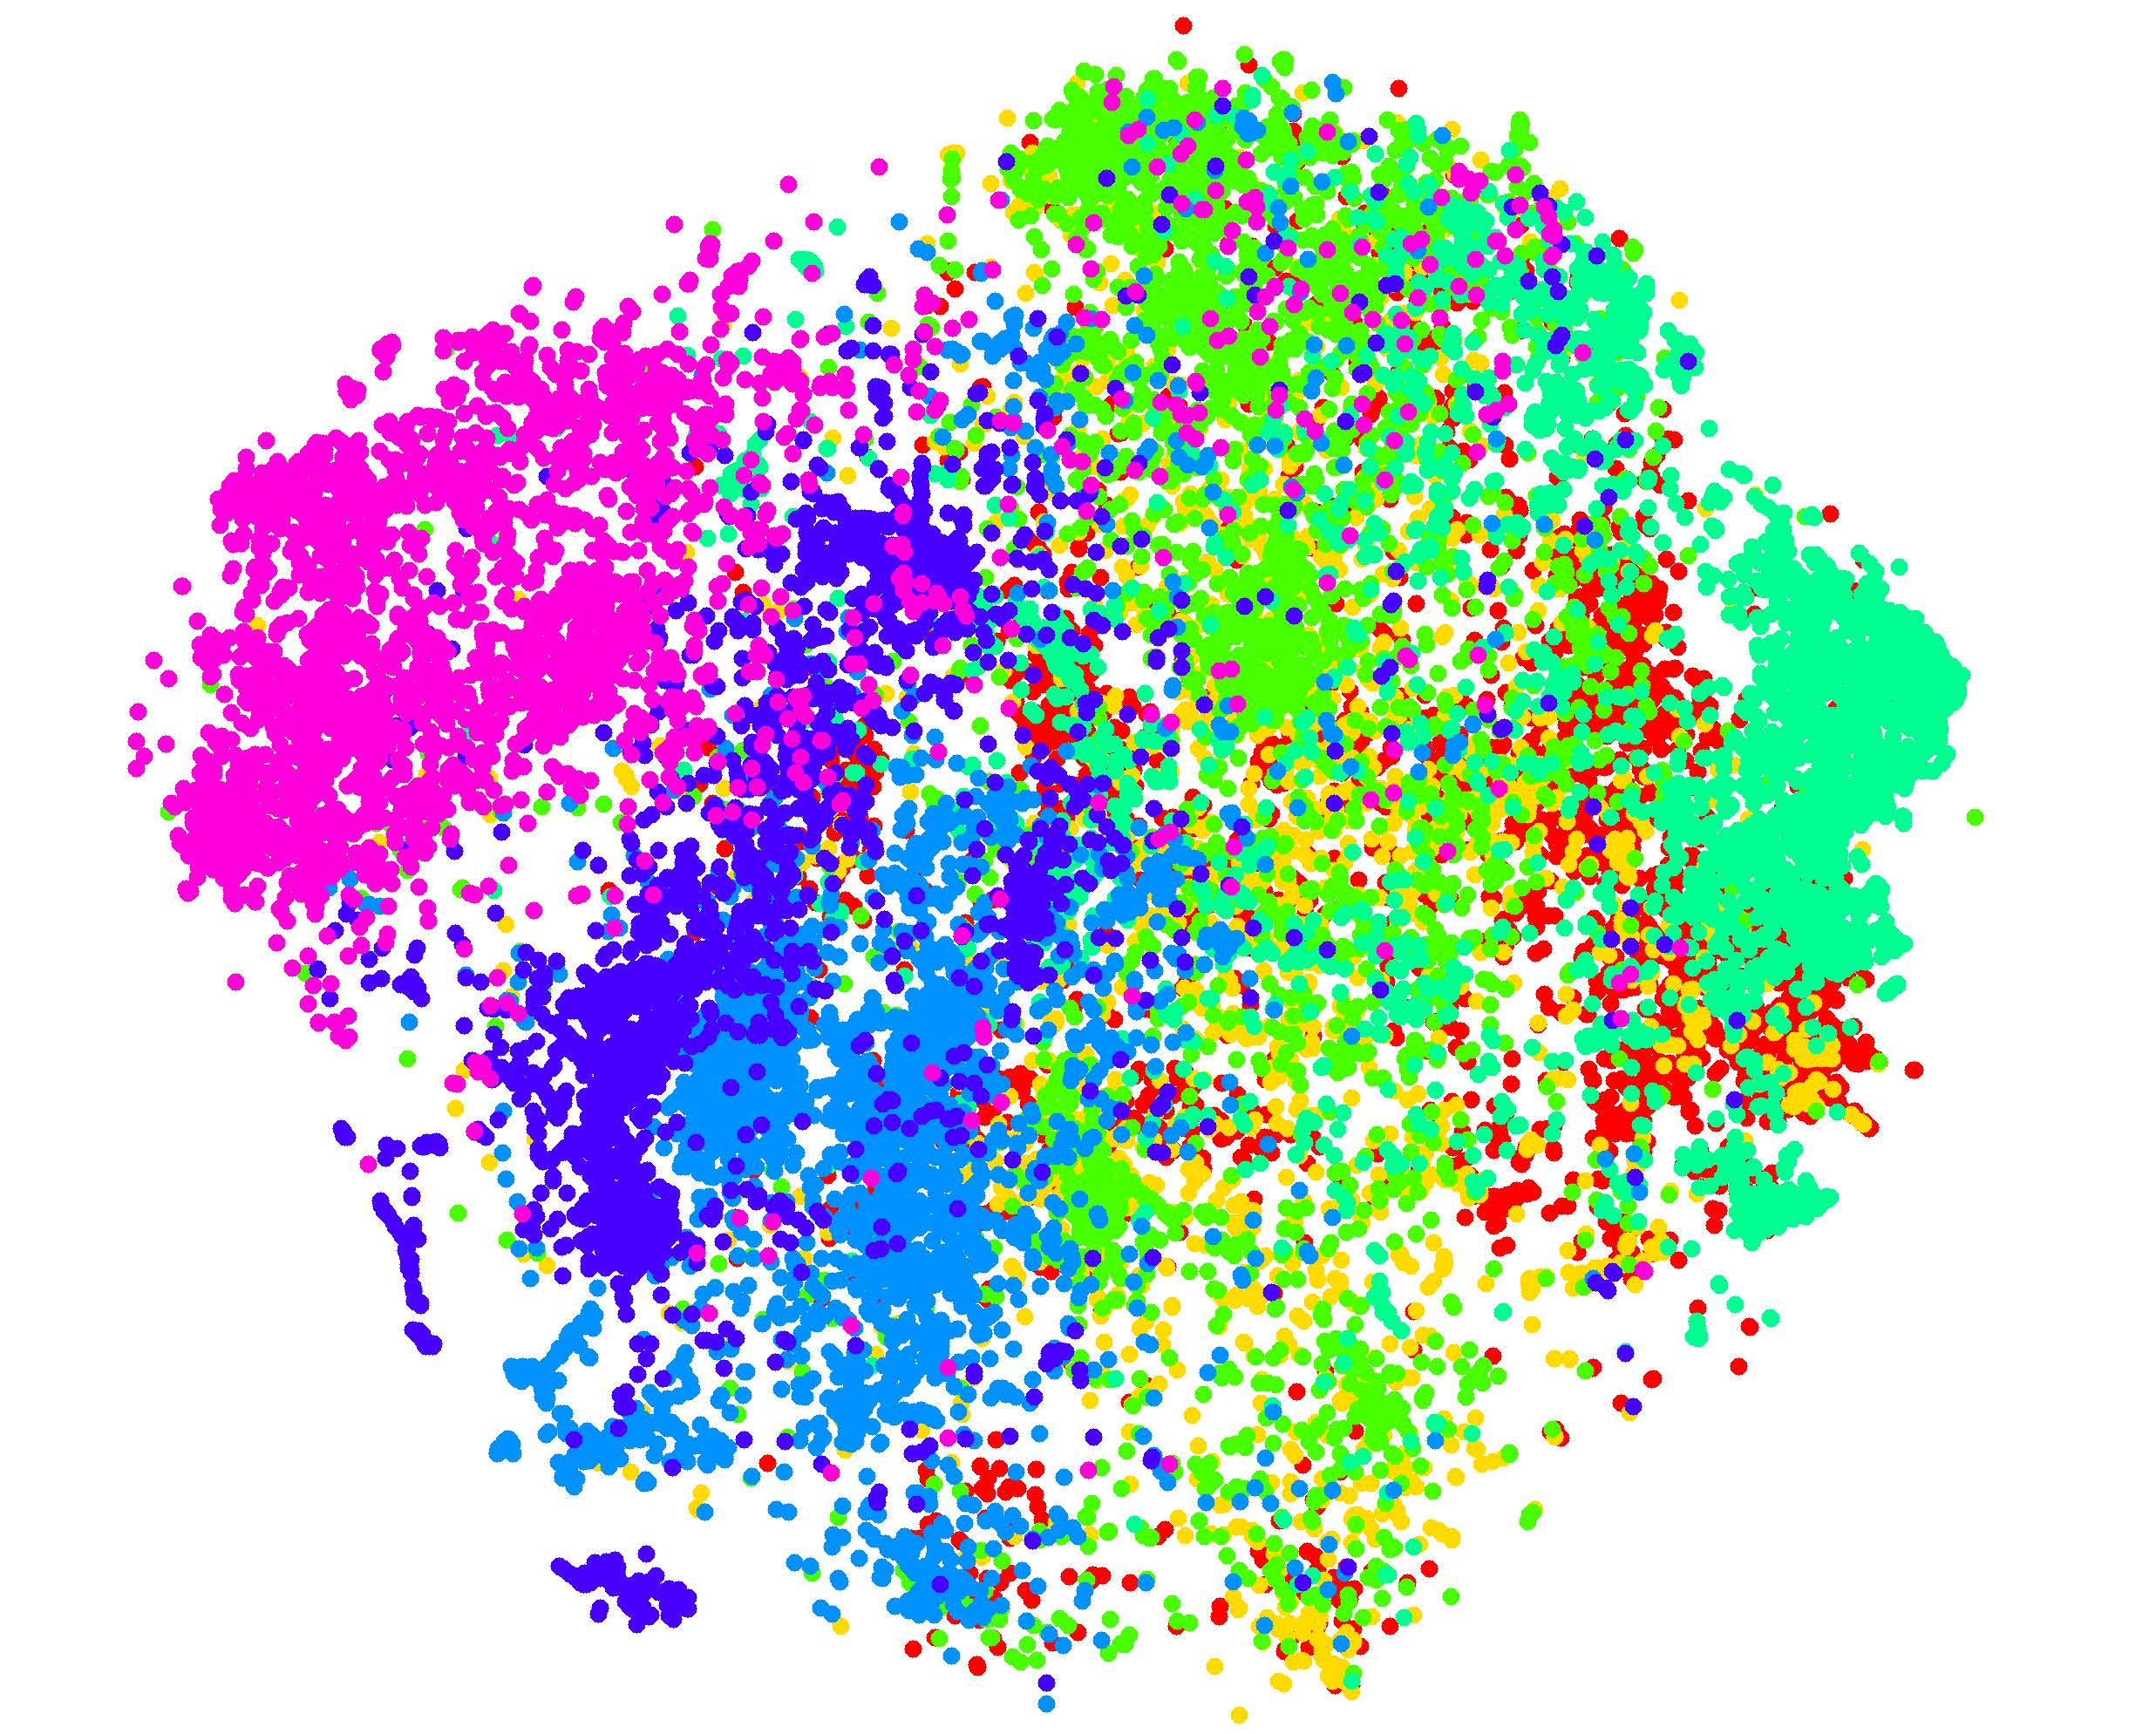
\includegraphics[width=0.3\textwidth]{DECAF6.jpg}}
\caption{这是标题}
\label{thisiisalabel}
\end{figure}

使用服务

您必须遵守服务中提供的所有政策。

请勿滥用我们的服务。举例而言,请勿干扰我们的服务或尝试使用除我们提供的界面和指示以外的方法访问这些服务。您仅能在法律(包括适用的出口和再出口管制法律和法规)允许的范围内使用我们的服务。如果您不遵守我们的条款或政策,或者我们在调查可疑的不当行为,我们可以暂停或停止向您提供服务。

\section{插入章节}
\esection{Insert Sections}

\subsection{二级章节}
\esubsection{Subsection}

使用我们的服务并不让您拥有我们的服务或您所访问的内容的任何知识产权。除非您获得相关内容所有者的许可或通过其他方式获得法律的许可,否则您不得使用服务中的任何内容。本条款并未授予您使用我们服务中所用的任何商标或标志的权利。请勿删除、隐藏或更改我们服务上显示的或随服务一同显示的任何法律声明。

我们的服务会显示一些不属于 Google 的内容。这些内容由发布的实体承担全部责任。我们可能会审查相关内容,以确定其是否违法或违反了我们的政策;如果我们有理由相信该内容违反了我们的政策或违法,我们可以将其删除或拒绝显示。不过,这并不意味我们必然会审查内容,因此请勿想当然地认为我们在进行审查。

在您使用服务的过程中,我们可能会向您发送服务公告、管理消息和其他信息。您可以选择不接收上述某些信息。

我们的部分服务可在移动设备上使用。在使用此类服务时,请勿因此而分散注意力和违反交通或安全法。

\section{插入表格}
\esection{Insert Tables}

\begin{table}[htbp]
\centering
\caption{表格示例}\label{TABfeatures}
\begin{tabular}
{ccccccc}
\toprule
Colorhist& GETLF& GIST& SIFT& C-SIFT& RGB-SIFT& OPPONENT-SIFT\\
\hline
576& 256& 480& 5000& 5000& 5000& 5000\\
\bottomrule
\end{tabular}
\end{table}

为了使用我们的某些服务,您可能需要一个 Google 帐户。您可以创建自己的 Google 帐户或者由管理员(例如您所在的单位或教育机构)为您分配 Google 帐户。如果您使用的是由管理员分配的 Google 帐户,可能需要遵守另外的条款或附加条款,并且您的管理员可能有权访问或停用您的帐户。

为保护您的 Google 帐户,请务必保管好您的密码并对外保密。您应对自己 Google 帐户上发生的活动或通过该帐户进行的活动负责。尽量不要在第三方应用中使用与 Google 帐户相同的密码。如果您发现有人在未经授权的情况下使用了您的密码或 Google 帐户,请按这些指示操作。

\section{插入公式}
\esection{How to Insert an Equation}

\begin{equation}\label{EQKeywordWeight}
s(t_n) = \frac{1}{\sum_{\forall t\in\tau}s(t)} \sum_{\forall t_{n,m}\in\tau}F_{n,m}\mathrm{sigm}(\mathrm{d}_{n,m})
\end{equation}

\section{插入列表}
\esection{How to Insert an List}

我们会根据美国《数字千年版权法》规定的流程,对涉嫌侵犯版权的通知作出回应并终止屡次侵权人的帐户。

我们会向版权持有人提供信息,以帮助他们在线管理自己的知识产权。如果您认为有人侵犯了您的版权并希望通知我们,可以在我们的帮助中心内查阅有关提交通知的信息和 Google 关于回应通知的政策。

\begin{enumerate}

\item 条目 1。
\item 条目 2(第 $n_l$ 层),计算:

        $$
        \delta^{(n_l)} = - (y - a^{(n_l)}) \bullet f'(z^{(n_l)})
        $$ 

\item 对于 $l = n_l-1, n_l-2, n_l-3, \ldots, 2$ 的各层。
\item 条目 4。

        \[ 
        \begin{aligned}
        \nabla_{W^{(l)}} J(W,b;x,y) &= \delta^{(l+1)} (a^{(l)})^T, \\
        \nabla_{b^{(l)}} J(W,b;x,y) &= \delta^{(l+1)} 
        \end{aligned}
        \]
\end{enumerate}

隐私与版权保护

Google 的隐私权政策介绍了您在使用我们的服务时,我们会如何处理您的个人数据和保护您的隐私。使用我们的服务即表示您同意 Google 可以按照我们的隐私权政策使用您的个人数据。

我们会根据美国《数字千年版权法》规定的流程,对涉嫌侵犯版权的通知作出回应并终止屡次侵权人的帐户。

我们会向版权持有人提供信息,以帮助他们在线管理自己的知识产权。如果您认为有人侵犯了您的版权并希望通知我们,可以在我们的帮助中心内查阅有关提交通知的信息和 Google 关于回应通知的政策。

\section{图片表格混合插入}
\esection{Mix with Images and Tables}

文字多时,使用\verb|\tabincell|进行插入。注意需要使用手动\\
换行。

\begin{table}[htbp]
\centering
\caption{图片表格混合插入}\label{TABBP1resultdemo}
\begin{tabular}
{cll}
\toprule
类别      &示例图片1  &示例图片2  \\
\hline
图像&
\tabincell{c}{
\includegraphics[width=0.35\textwidth]{9ddQpU7yeNmEzUXu.jpg}\\9ddQpU7yeNmEzUXu.jpg} &
\tabincell{c}{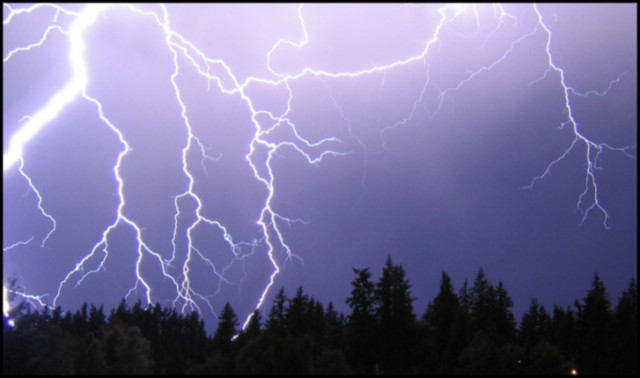
\includegraphics[width=0.42\textwidth]{9_cX52_TUIjODdac.jpg}\\9\_cX52\_TUIjODdac.jpg} \\

\hline

\tabincell{c}{Ground\\Truth} &
\tabincell{l}{keywords keywords\\
keywords keywords} &
\tabincell{l}{keywords 垂直居中} \\

\bottomrule
\end{tabular}
\end{table}

\section{插入引用}
\esection{How to Insert a Citation}

引用公式\ref{EQKeywordWeight}。

引用图片\ref{thisiisalabel}。

引用表格\ref{TABfeatures}。

引用参考文献\cite{smeulders2000content}。
